\documentclass[journal,12pt,twocolumn]{IEEEtran}
\usepackage{amsmath,amssymb,amsfonts,amsthm}
\usepackage{txfonts}
\usepackage{tkz-euclide}
\usepackage{listings}
\usepackage{gvv}
\usepackage[latin1]{inputenc}
\usepackage{array}
\usepackage{pgf}
\usepackage{lmodern}

\begin{document}
\bibliographystyle{IEEEtran}

\vspace{3cm}

\title{}
\author{EE23BTECH11054 -  Sai Krishna Shanigarapu$^{*}$
}
\maketitle
\newpage
\bigskip

% \renewcommand{\thefigure}{\theenumi}
% \renewcommand{\thetable}{\theenumi}

\section*{Exercise 9.2}

\noindent \textbf{13} \hspace{2pt}If the sum of $n$ terms of an A.P. is $3n^2+5n$ and its $m^{th}$ term is 164, find the value of $m$.
\bigskip

\solution:
\noindent
\begin{align}
Y\brak{z} &=  \sum_{n=0}^{\infty} y\brak{n}z^{-n} \\
&= \frac{2\brak{4-z^{-1}}}{\brak{1-z^{-1}}^3}, \qquad |z| > 1\\
U\brak{z} &= \frac{1}{1-z^{-1}}, \qquad |z| > 1\\
X\brak{z} &=  \frac{Y\brak{z}}{U\brak{z}}\\
x\brak{n} &= Z_{z}^{-1}\left[2\left(\frac{1}{1-z^{-1}}\right) + 6\left(\frac{1}{1-z^{-1}}\right) ^2\right]
\end{align}

%In order to compute the Z-inverse of \begin{align} X\brak{z} &= (1-z^{-1})^{-2} \end{align} we develop the Power series for the function\\ $(1-x)^{-2}$.
%\begin{align}\brak{1-x}^{- \brak{\beta + 1}} &= \sum_{n=0}^{\infty} \binom{n+\beta}{\beta}x^n \end{align}
%for $x=z^{-1}$ and $\beta = 1$,
%\begin{align}(1-z^{-1})^{-2} = \sum_{n=0}^{\infty} \binom{n+1}{1} z^{-n}\end{align}
%Comparing with the definition of $Z-$transform,\\
%\begin{align}
 %   Z_{z}^{-1}\left(\frac{1}{1-z^{-1}}\right)^2 &= \brak{n+1}\brak{u\brak{n}}\\
 %   x\brak{n} &= \brak{6n+8}\brak{u\brak{n}}\\
 %   164 &= \brak{6m+8}\brak{u\brak{n}}\\
 %   m &= 26
%\end{align}
The inverse $Z-$transform of $\brak{1-z^{-1}}^{-2}$ using Contour integration is given by,
\begin{align}
    Z_z^{-1} &= \frac{1}{2\pi j}\oint_C X\brak{z}z^{n-1}dz\\
    &= \frac{1}{2\pi j}\oint_C \frac{z^{n+1}}{\brak{z-1}^2}\\
    &= \frac{1}{\brak{2-1}!}\left[ \frac{d}{dz}\left(\brak{z-1}^2 \frac{z^{n+1}}{\brak{z-1}^2}\right) \right]_{z=1}\\
    &= \brak{n+1}\brak{u\brak{n}}\\
    x\brak{n} &= \brak{6n+8}\brak{u\brak{n}}\\
    164 &= \brak{6m+8}\brak{u\brak{n}}\\
    m &= 26
\end{align}

\setlength{\arrayrulewidth}{0.3mm}
\setlength{\tabcolsep}{15pt}
\renewcommand{\arraystretch}{1.4}

\begin{table}[ht]
\centering

\begin{tabular}{|c|c|}
\hline

\textbf{Symbol} & \textbf{Remarks}\\
\hline
$y\brak{n} =\brak{3n^2+11n+8}\brak{u\brak{n}}$ & Sum of $n$ terms  \\
\hline
$x(m-1)$ & $164$\\
\hline
$y\brak{n}$ & $x\brak{n} * u\brak{n}$\\
\hline
$Z_{z}^{-1}\brak{1-z^{-1}}^{-2}$ & $u\brak{n}$\\
\hline

\end{tabular}
\vspace{0.25cm}
\caption{Parameters}
%\label{tab:11.9.2.13.1}



\end{table}



\begin{figure}[htbp]
    \centering
    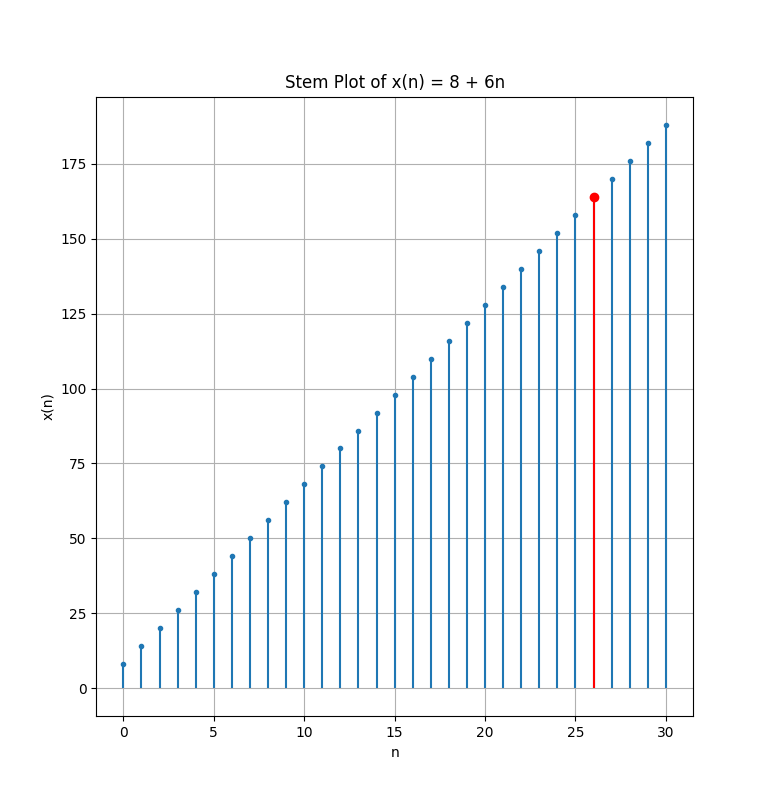
\includegraphics[width=1.0\columnwidth]{figs/Figure_1.png}
    \caption{Plot of x(n) vs n}
    \label{fig:11.9.2.13.1}
\end{figure}

%\setlength{\arrayrulewidth}{0.3mm}
\setlength{\tabcolsep}{15pt}
\renewcommand{\arraystretch}{1.4}

\begin{table}[ht]
\centering

\begin{tabular}{|c|c|}
\hline

\textbf{Symbol} & \textbf{Remarks}\\
\hline
$y\brak{n} =\brak{3n^2+11n+8}\brak{u\brak{n}}$ & Sum of $n$ terms  \\
\hline
$x(m-1)$ & $164$\\
\hline
$y\brak{n}$ & $x\brak{n} * u\brak{n}$\\
\hline
$Z_{z}^{-1}\brak{1-z^{-1}}^{-2}$ & $u\brak{n}$\\
\hline

\end{tabular}
\vspace{0.25cm}
\caption{Parameters}
%\label{tab:11.9.2.13.1}



\end{table}


\end{document}
